%!TEX root = ../trajectory-grouping.tex
\begin{wrapfigure}[19]{r}[1.5cm]{.4\textwidth}
    \Centering\vspace{-\baselineskip}
    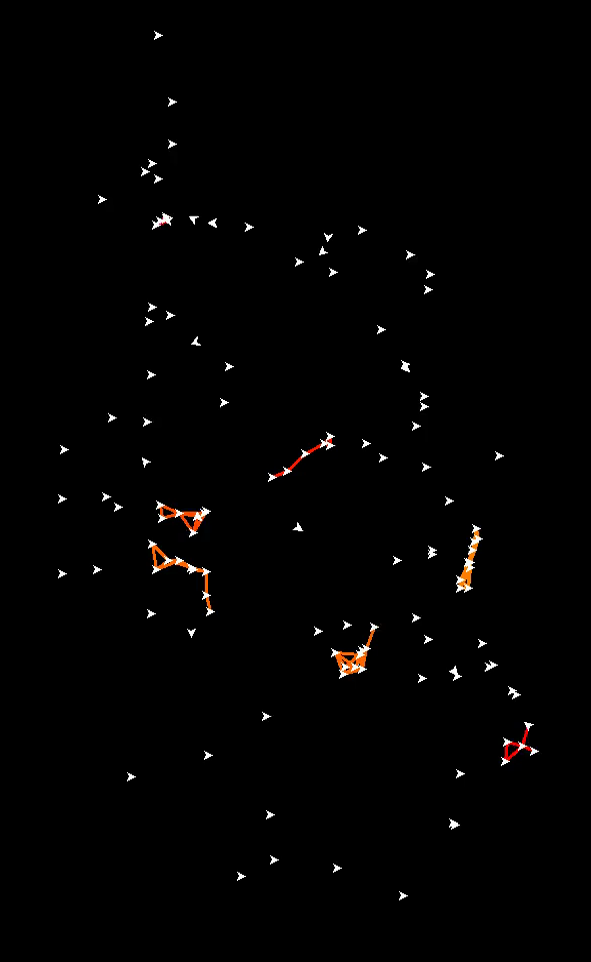
\includegraphics[width=.35\textwidth]{Bilder/starkey.png}
    \renewcommand{\figurename}{Abb.}
    \caption{Screenshot aus dem Video zu den Starkey-Daten, \cite{starkey-video}.}\label{fig:starkey}
\end{wrapfigure}
Da das Ziel darin bestand, menschliche Intuition in ein mathematisches Modell zu überführen, haben \textcite{buchin2015} das Modell implementiert, auf unterschiedliche Testdaten angewandt und zur Visualisierung Videos produziert,\footnote{verfügbar unter \url{https://fstaals.net/grouping/}} an denen man gut überprüfen kann, ob dieses Ziel erreicht wurde.
Eine Menge von Trajektorien wurde dabei synthetisch basierend auf dem NetLogo-Modell  \cite{netlogo} erstellt, die zweite ist eine Teilmenge von Positionsdaten aus dem Starkey-Projekt \cite{starkey}, die die Bewegung von Hirschen, Elchen und Rindern im \emph{Starkey Experimental Forest} in Oregon erfassen.
Diese Daten mussten zu diesem Zweck interpoliert werden, um die \cref{sec:trajek_reeb} eingeführten Bedingungen zu erfüllen.

Bei beiden Datensets zeigt sich, dass das Modell der menschlichen Intuition sehr gut entspricht.
\Cref{fig:starkey} zeigt einen Screenshot aus dem Video zu den Starkey-Daten, was dies schon verdeutlich -- erst in bewegten Bildern wird insbesondere die Einwirkung von $\delta$ aber wirklich klar.
Ohne zu wissen, was die Enitäten für Arten sind, zeigt sich deutlich, dass die Tiere zumindest teilweise ein Herdenverhalten zeigen.
Die Videos mit den NetLogo-Daten belegen außerdem gut, wie die in \cref{cha:def_gruppe} besprochene Monotonie bei Variation der Parameter zum Tragen kommt.

\section{Weiterführende Themen}
\begin{figure}[tp]
    \Centering
    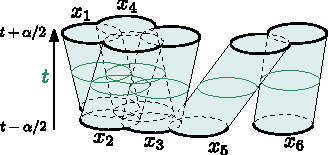
\includegraphics[width=.5\textwidth]{Bilder/alpha-component}
    \caption{eine $\alpha$-Komponente zum Zeitpunkt $t$, \cite[Fig:~11]{buchin2015}}\label{fig:alpha}
\end{figure}
Das hier betrachtete Modell zur \emph{Trajectory Grouping Structure} lässt sich über die besprochenen Aspekte hinaus noch weiter verbessern, was an dieser Stelle stichpunktartig erläutert werden soll:
\begin{description}
    \item[Höhere Dimensionen] Ein genauerer Blick auf das Modell zeigt, dass es nicht nur für Bewegungen in der Ebene geeignet ist, sonder prinzipiell auch in höheren Dimensionen benutzt werden kann -- der zweidimensionale Fall ist, wenn man GPS-Daten verarbeiten will, aber selbstverständlich das Hauptanwendungsgebiet.
    \item[Robuste Gruppen] In \textcite[Sec.~4]{buchin2015} wird das Modell noch etwas verfeinert, um weniger anfällig gegenüber gestörten Daten zu sein.
    Dazu führen \textcite{buchin2015} einen weiteren Parameter $\alpha$ ein, der die maximale Dauern einer Störung angiebt.
    Dieser findet nun in einer modifizierten Definition von \emph{direkt zusammenhängend} Anwendung:
    
    \begin{definition}
        Zwei Entitäten heißen \bet{$\alpha$-approximativ direkt zusammenhängend}\index{$\alpha$-approximativ direkt zusammenhängend@approximativ direkt zusammenhängend} zum Zeitpunkt $t$, falls sie direkt zusammenhängend zu einem Zeitpunkt $t' \in \benbrace*{t- \alpha/2, t+ \alpha/2}$ sind.\index{direkt zusammenhängend}
    \end{definition}
    
    Eine Komponente kann dann zum Beispiel so aussehen, wie in \cref{fig:alpha}, insbesondere müssen in einer Komponente zum Zeitpunkt $t$ die $t'$ nicht alle übereinstimmen!
    Den zugehörigen Reeb-Graph kann man nun aus dem Reeb-Graph der ursprünglichen Definition berechnen, indem man ihn sukzessive \enquote{vereinfacht}, dabei kann zum Beispiel ein Split-Knoten und ein direkt nachfolgender Merge-Knoten durch eine einzige Kante ersetzt werden, wenn dieses Aufteilen der Komponenten nicht zu lange andauert.
    Dies führt insgesamt zu einem Algorithmus mit Laufzeit $\mathcal{O}(\tau n^3 \log n + N)$, wobei $N$ wieder die Größe der Ausgabe ist, \cite[Thm.~13]{buchin2015}.
    \item[Verbesserte Definition] Durch \textcite{grouping_improved} wurde die Definition einer Gruppe aus \textcite{buchin2015} mittlerweile weiter verbessert.
    Bei sehr dichten Mengen von Entitäten können noch Fälle eintreten, die nicht der menschlichen Intuition entsprechen, da Entitäten dann $\varepsilon$-zusammenhängend über eine Kette von Entitäten sein können, die aber gar nicht zu den Gruppe gehören.
    In \textcite{grouping_improved} wird folglich \cref{enum:3:def:gruppe} aus \cref{cha:def_gruppe} entsprechend modifiziert, was natürlich auch neue Algorithmen nötig macht.
    \textcite{grouping_improved} geben dazu zwei Algorithmen an, einen mit einer Laufzeit von $\mathcal{O}(\tau^2 n^5 \log n)$, den anderen mit $\mathcal{O}(\tau n^4 2^n)$.
    Letzterer kann trotz exponentieller Komplexität in $n$ deutlich performanter sein, wenn $\tau \gg n$.
\end{description}

\section{Fazit}
Zusammenfassend lässt sich sagen, dass \textcite{buchin2015} ein stimmiges Modell zu Gruppierung von Trajektorien geliefert haben, was sich vor allem durch die hohe Übereinstimmung mit der menschlichen Intuition kollektiver Bewegungen auszeichnet.
Durch das Benutzen topologischer Methoden (Betrachtung von Zusammenhangskomponenten, Reeb-Graph) entstehen dabei einige Vorteile gegenüber anderen Modellen zur Gruppierung, die über den Vorteil einer relativ intuitiven Definition von Gruppen hinausgehen: Das \enquote{Leben} der Gruppen lässt sich detailliert erfassen und die Zeitpunkte, an denen dies geschieht, sind nicht auf die Zeitstempel der Trajektorien eingeschränkt.
